\documentclass[10pt]{beamer}

\usetheme[progressbar=frametitle]{metropolis}
\usepackage{appendixnumberbeamer}

\usepackage{comment}

\usepackage{booktabs}
\usepackage[scale=2]{ccicons}

\usepackage{pgfplots}
\usepgfplotslibrary{dateplot}

\usepackage{xspace}
\newcommand{\themename}{\textbf{\textsc{metropolis}}\xspace}

\usepackage{listings}

\metroset{block=fill}


\title{Programmeringstävling Nao}
\subtitle{Mattekollo}
\date{4e Augusti 2018}
%\date{}
\author{Fredrik Löfgren, Jinci Brettschneider, Jonatan Nilsson}
%\institute{Mattekollo}
% \titlegraphic{\hfill
\includegraphics[height=1.5cm]{logo.pdf}}

\begin{document}

\maketitle

\begin{frame}{Innehåll}
  \setbeamertemplate{section in toc}[sections numbered]
  \tableofcontents[hideallsubsections]
\end{frame}

\section{Regler}

\begin{frame}[fragile]{Vad får man använda?}

\begin{itemize}
\item Bara python 3.7 får användas (det som är installerat på skoldatorerna).
\item Inga andra bibliotek än de som finns på skoldatorerna (matplotlib, numpy, arcade är installerat förutom standard python) får användas. Vid tveksamheter ska vi kunna testa på en elevdator. Ni får självklart testa på såna i era grupper. 
\item Internet är tillåtet, men du måste kunna förklara din kod och svara på våra frågor för att få poäng. Du får inte sno \emph{hela} lösningar från nätet. Upptäcker vi fusk på någon uppgift kan ni inte få poäng på den uppgiften. 
\item Det är tillåtet att anteckna andras lösningar när de presenterar på tavlan, dels för att lära sig men också för att implementera deras algoritm smartare och tjäna mer poäng
\end{itemize}
\end{frame}

\begin{frame}[fragile]{Vilka jobbar?}

\begin{itemize}
\item Ni jobbar i grupper om 3 så långt det är möjligt. 
\item Vi har delat upp grupperna. 
\item Vi lärare kommer inte kunna hjälpa er med någon programmering, ni får fråga varandra i gruppen istället. Det enda vi kan svara på är frågor relaterat till problemformuleringarna. 
\end{itemize}
\end{frame}



\begin{frame}[fragile]{Hur fungerar tävlingen?}

\begin{itemize}
\item Ni får ett problem presenterat på projektorn. Det är relativt enkelt och vi bedömer att det i snitt tar 10 minuter att lösa på egen hand, men förhoppningsvis snabbare i grupp. 
\item Den som är klar med sin lösning först säger till oss ledare genom att skrika sitt gruppnamn. Då måste de släppa sina datorer och inte koda något mer. 
\item Gruppen som har en lösning får gå fram till tavlan och koppla in sin dator och starta sitt program. Sen kommer en ledare att testa det med testfall som vi bestämmer. Programmet ska gå att förstå och använda för oss (behöver inte vara snyggt).
\item Om programmet klarar testfallen så ska ni presentera er kod för de andra deltagarna. Om det inte fungerar / klarar testfallen får ni gå och sätta er igen utan att presentera er kod. 
\end{itemize} 
\end{frame}




\begin{frame}[fragile]{Poängräkning?}

\begin{itemize}
\item Om ni inte kan förklara er kod tillräckligt bra (bedöms av lärarna) så får ni 0 poäng för det försöket. Ingen annan får heller poäng. 
\item Om ni har rätt på testfallen och kan förklara er kod får ni 100 poäng. 
\item Om programmet tar mer än ca 30s att köra, så får ni 0 poäng. Våra exempellösningar går oftast på $\le1$s.
\item Om ni har fel på testfallen så får alla andra tävlande lag 100 poäng. Detta för att ni inte ska chansa och gå fram för tidigt och slösa vår värdefulla tid. 
\end{itemize}
\end{frame}



\begin{frame}[fragile]{Poängräkning - special!}

\begin{itemize}
\item Vissa lag kanske bara hade någon rad kvar innan ett annat lag blev klara och fick presentera. Istället för att slänga bort allt ert fantastiska arbete så ger vi er chansen att visa upp det och ändå få poäng, under förutsättning att er kod är kortare (färre bytes) än de som tidigare presenterat. 
\item Vi är medvetna om att kort kod inte alltid betyder bra kod, men det är enklare att mäta än tidsåtgången då ni kör på olika datorer. Dessutom finns det många tävlingar där man ska skriva så kort kod som möjligt.
\end{itemize}

\end{frame}




\begin{frame}[fragile]{Poängräkning - special!}

\begin{itemize}
\item För en korrekt visad lösning som ni kan förklara får ni hälften av poängen som delades ut innan på den här uppgiften.  
\item För en lösning som inte klarar testfallen så får alla andra lagen hälften av det som delades ut innan på den här uppgiften. 
\item Ni kan fortsätta att förkorta lösningar och få hälften av poängen igen. Men ni kan aldrig presentera igen på en uppgift som ni redan klarat testfallen på (oavsett om ni kunde förklara er kod och fick full poäng, eller inte klarade och fick 0 poäng). Har ni däremot haft fel på testfallen, och gett alla andra lag poäng, kan ni fortsätta testa på den uppgiften.
\end{itemize}
\end{frame}




\begin{frame}[fragile]{Hur fortsätter det?}

\begin{itemize}
\item Varje gång någon har klarat testfallen och presenterat korrekt för ett problem så kommer vi släppa ett nytt problem på projektorn. Vi presenterar inte ett nytt problem när någon lyckas visa en ny kortare lösning på ett redan avklarat problem.
\item Ni får fota eller skriva av problemformuleringen för vi kan inte gå fram och tillbaka mellan problemen hela tiden. 
\item Ni får alltså fler och fler problem att lösa, och ni kan alltid fortsätta att försöka på problem som ni tidigare inte klarat för att lyckas få halva poäng (vilket fortfarande är rätt mycket!).
\end{itemize}
\end{frame}





\begin{frame}[fragile]{Exempel!}

\begin{itemize}
\item Vi har lag A, B, C.  De får ett problem I. 
\item Lag C säger att de klarat uppgiften och går fram och presenterar, de lyckas både med testfall och att förklara sin kod och får 100 poäng. 
\item Ett problem II presenteras och lag B delar upp sig så att två personer satsar på det nya medan en fortsätter med problem I. Lag A förstår inte det nya problemet så alla sitter kvar med problem I. 
\item Lag A skriker att de är klara och får presentera sitt problem. De lyckas och får 50 poäng. Inget nytt problem presenteras då problem I redan är löst.
\item Lag B är klara med problem II, de lyckas med alla testfall och presentationen och får därmed sina första 100 poäng! 
\item Problem III presenteras.
\item Lag B säger att de är klara med problem III, men har tyvärr fel och ger alla andra lag 100 poäng. Inget nytt problem presenteras då. 
\item Lag B säger igen att de är klara, nu på problem I som en ensam stackare jobbat på. De lyckas med testfallet och får 25 poäng! 
\end{itemize}
\end{frame}





\begin{frame}[fragile]{Frågor?!}

Något som är oklart innan vi sätter igång? 

\end{frame}




\section{Då börjar vi!}

\begin{frame}{Baklängesmeningar}
Skriv en kod som vänder på en mening. Om jag skriver in "Jag heter Fredrik" ska programmet skriva ut "Fredrik heter Jag". Programmet ska ta in information med hjälp av input() och skriva ut meningen med print(). 

\end{frame}








\begin{frame}{FizzBuzz problemet}
FizzBuzz var från början en lek för barn för att lära sig vilka tal som är delbara med tre och fem, men har på senare tid blivit ett vanligt problem som man får på anställningsintervjuer när man sökt jobb som programmerare på Google eller Microsoft. 

Skriv ett program som skriver ut talen 1 till 100. Men för alla tal som är multiplar av tre skriver det ut ''Fizz'' istället för talet, och för alla multiplar av fem skriver det ut ''Buzz''. För tal som är en multipel av både fem och tre ska ''FizzBuzz'' skrivas ut istället. 
\end{frame}


\begin{frame}{Recept}

Du har bestämt dig för att laga mat. För att laga maten behöver du $N$ ingredienser. För varje ingrediens vet du hur mycket du redan har hemma, hur mycket du behöver totalt samt kostnaden för ingrediensen om du måste köpa den. Du skall alltså köpa den mängd av varje ingrediens som du saknar. Uppgiften är att beräkna kostnaden för att laga maten. Det kommer inte finnas mer än 5 ingredienser.

Programmet ska fråga efter antalet ingredienser och sedan för varje ingrediens hur mycket du redan har hemma, hur mycket du behöver totalt samt hur mycket den kostar (per enhet) om du måste köpa den. Programmet ska skriva ut den totala kostnaden. 

\end{frame}






\begin{frame}{ISNT + THIS + FUN = STUFF}

ISNT + THIS + FUN = STUFF

Ersätt varje bokstav med en unik siffra (0-9) så att ekvationen stämmer. Observera att första talet i siffran inte kan vara 0. Skriv ut alla tal STUFF kan representera för att ekvationen ska stämma. 

\end{frame}





\begin{frame}{Summerbar lista}

Skriv ett program som tar in en lista av heltal på en rad, och ett ensamt heltal $N$ på nästa rad. Ta reda på om man kan bilda talet $N$ som en summa av två tal från listan. Om det är möjligt så skriv ut de två talen (om det finns flera lösningar, skriv ut alla), annars skriv ut att det är omöjligt.

\end{frame}





\begin{frame}{Bankkortsnummer}

De flesta bankkortsnummer, och många andra nummer för säkerhet, kan valideras med en algoritm som Hans Peter Luhn på IBM har utvecklat. Han beskriver sin algoritm i patent US2950048 från 1954 (mjukvarupatent är ingenting nytt!). Luhns algoritm hittar nästan alla fel när man råkat skriva fel siffra på ett ställe i talet, och alla gånger man har råkat byta plats på två siffror bredvid varandra utom fallet 09 och 90. 

Luhn algoritmen jobbar från höger till vänster, med siffran längst till höger som kontrollsiffra. Varannan siffra, med start på den siffra längst till vänster, ska dubbleras. Sen adderar man ihop siffersumman av alla tal, både de dubblade och de odubblade. Numret är ett giltigt bankkortsnummer om summan är jämnt delbar på 10. 

Skapa ett program som validerar bankkortsnummer, be användaren om ett tal och skriv ut om det är giltigt eller ej. 

\end{frame}

\begin{comment}
For example, the number 49927398716 is valid according to the Luhn algorithm. Starting from the right, the sum is 6 + (2) + 7 + (1 + 6) + 9 + (6) + 7 + (4) + 9 + (1 + 8) + 4 = 70, which is divisible by 10; the digit-sums of the doubled digits have been shown in parentheses.
\end{comment}



\begin{frame}{Veckodag}

Be användaren om ett årtal, en månad och ett datum. Beräkna vilken veckodag det datumet är och skriv ut dagen med bokstäver på svenska. 

\end{frame}


\begin{frame}{Dubbla differensen}
Givet ett tal $n$, skriv ut den positiva skillnaden mellan talet $n$ och 21, förutom om $n$ är större än 21, då ska du skriva ut dubbla positiva differensen. 


\begin{exampleblock}{Indata}
Ett positivt heltal $n$.
\end{exampleblock}

\end{frame}







\begin{frame}{Uppochnedvända tal}

Ett uppochnedvänt tal är ett tal som ser ut att vara likadant om man läser uppochned, åtminstone om man läser lite snabbt och slarvigt. Till exempel är 689 och 1961 uppochnedvända tal. Dessa siffror räknas som uppochnedbara siffror: 0, 1, 6, 8, 9 

\begin{exampleblock}{Indata}
Ett heltal $N$, som alltid är mindre än 10 000.
\end{exampleblock}

\begin{exampleblock}{Utdata}
Skriv ut antalet uppochnedvända tal som finns från 0 till $N$.
\end{exampleblock}

\end{frame}





\begin{frame}{Utan max()}
Skriv ett program som tar in tre heltal och skriver ut det största av de tre. Du får inte använda den inbyggda funktionen max() i python. 
\end{frame}




\begin{frame}{Kängurumamman}
 En kängurumamma ska packa ner sina barn i sin pung. Hon har massor med barn. De två minsta väger bara ett gram var men sen väger varje barn lika mycket som de två föregående tillsammans. Hennes sex minsta barn väger alltså 1, 1, 2, 3, 5 och 8 gram. Mamman orkar bära högst X kilo (och inte ens ett gram mer). Hur många barn kan hon ta med sig?

\begin{exampleblock}{Indata}
Ett heltal $X$, där $1{\le}X\le1000$, det maximala antalet kilo mamman orkar bära. 
\end{exampleblock}
\begin{exampleblock}{Utdata}
Programmet ska skriva ett heltal, det största antalet barn som tillsammans väger högst $X$ kilo. 
\end{exampleblock}

\end{frame}

\begin{frame}{Jincis sorti}

Jinci kom fyra i Genikampen 2016, hon åkte ut i finalavsnittet på en uppgift där man skulle bilda torn av bokstavstärningar. Hon hade fem tärningar med vardera bokstäverna: 

\begin{itemize}
\item S, F, T, N
\item M, Y, O, Y
\item N, A, S, B
\item I, R, E, G
\item K, L, T, D
\end{itemize}

Vilka ord kan hon bilda av dessa bokstäver? Du behöver inte ta hänsyn till bokstävernas inbördes relation på varje tärning. 

Här har du en ordlista med svenska ord: \url{http://runeberg.org/words/ss100.txt}
(Kan behövas konvertera till utf-8)
%NOBEL
%FYSIK
%SMART
%TYNGD

\end{frame}

\begin{frame}{Romerska tal}

Skriv ett program som omvandlar romerska tal till tal skrivna med arabiska siffror.

De romerska talen skrivs enligt klassiska sättet, där till exempel IV motsvarar 4 medan VI motsvarar 6. Programmet ska inte hantera streck ovanför bokstäver (som i vissa sammanhang motsvarar multiplikation med 1000). 

\begin{exampleblock}{Indata}
Ett romerskt heltal mellan I och MMM.
\end{exampleblock}

\begin{exampleblock}{Utdata}
Ett heltal skrivet med arabiska siffror som motsvarar det romerska talet.
\end{exampleblock}

\end{frame}




\begin{frame}[fragile]{Leet speak}
Skriv ett program som översätter meningar från vanligt språk till leet speak. Leet speak är ett substitutionschiffer där varje bokstav i det vanliga alfabetet byts ut mot ett tecken i leet speak-alfabetet. Till din hjälp har du alfabetet för respektive språk:
\begin{verbatim}
vanligt:    abcdefghijklmnopqrstuvwxyz
leet speak: 48()3}6#!]X|MN09Q2Z7MVWXJZ
\end{verbatim}
Programmet ska läsa in en mening: en rad med tecken som kan vara a-z (stora eller små bokstäver) eller blanksteg. Programmet ska skriva ut meningen översatt till leet speak. 
\end{frame}



\begin{frame}{Glada tal}

Glada tal är definierade enligt följande: Börja med ett positivt heltal. Ersätt talet med summan av kvadraterna av dess siffror och repetera utförandet tills talet man har kvar är 1. Många tal blir aldrig 1 och fortsätter bara repetera processen i all oändlighet. Tal som slutar på 1 är glada tal och de som inte gör det är ledsna tal. Datorprogram som testar alla tal upp till och med $ 10^{20}$ visar på att ungefär 12\% av alla tal är glada tal, men det finns inget konkret bevis för det. 



\begin{exampleblock}{Indata}
Ett heltal $N$ som är 1000 som störst.
\end{exampleblock}

\begin{exampleblock}{Utdata}
Skriv ut alla glada tal som är strikt mindre än $N$.
\end{exampleblock}


\end{frame}



\begin{frame}{Digitala rötter}

Termen digital rot för heltalet $N$ innebär att man upprepade gånger summerar talets ingående siffror tills summan blir $\le10$. Till exempel för talet 34783 får man:
\vspace{-3mm}
$$3 + 4 + 7 + 8 + 3 = 25$$
$$2 + 5 = 7$$
Talet 34783 har digitala roten 7.

På liknande sätt kan man definiera digital produktrot för heltalet $N$, där man istället upprepade gånger multiplicerar ingående siffror tills produkten blir $\le10$. Till exempel för talet 34783 får man:
$$3 \cdot 4 \cdot 7 \cdot 8 \cdot 3 = 2016$$
$$2 \cdot 0 \cdot 1 \cdot 6 = 0$$
Talet 34783 har digital produktrot 0. Hos talet 34783 är alltså roten och produktroten olika.

Skriv ett program som tar reda på hur många tal i ett givet intervall som har samma digitala rot som produktrot.
\end{frame}




\begin{frame}[fragile]{Vindskydd}
Du ska bygga ett vindskydd längsmed en rektangels fyra kanter (med längden $L$ och bredden $B$) och ha höjden $H$.

De fyra vindskyddsväggarna skapas genom att skära upp ett platt rektangulärt plaststycke med dimensionerna $M \times N$ i fyra mindre bitar. Du skär alltid en gång parallellt med x-axeln och en gång parallellt med y-axeln, och du kan endast skära vid heltalskoordinater. Din uppgift är att bestämma på hur många olika godkända sätt man kan skära upp plasten. För att en skärning ska vara godkänd måste bitarna kunna täcka varsin vägg. Det gör ingenting om bitarna är för stora, men de får inte vara för små.

\vspace{-3mm}

  \begin{columns}[T,onlytextwidth]
    \column{0.5\textwidth}

\begin{exampleblock}{Indata}
Fem heltal: $L$, $B$, (där $L \geq B$), H, samt plaststyckets dimensioner M och N. Samtliga indatavärden är mellan 1 och 20, inklusive. 
\end{exampleblock}

    \column{0.5\textwidth}


\begin{figure}[!ht]
\centering
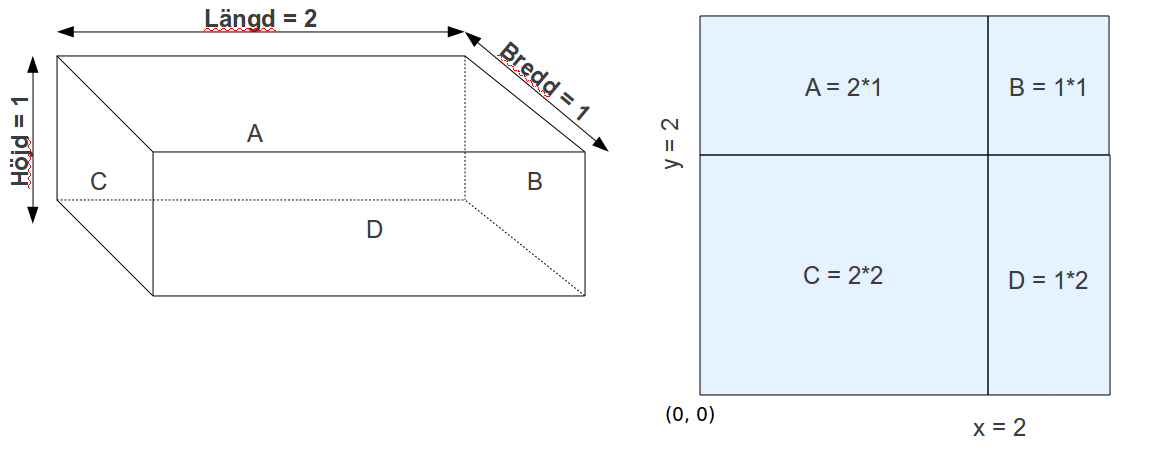
\includegraphics[width=\textwidth]{vindskydd}
%\caption{Figuren visar ett av sätten att skära plasten i körningsexempel 1. Observera att alla andra sätt att skära plasten (t.ex. vid $x=1$ och $y=1$) skapar en likadan uppsättning bitar, men de ska ändå räknas som olika skärningar.}
\label{fig:vindskydd}
\end{figure}

\end{columns}

%\begin{exampleblock}{Utdata}
%Programmet ska skriva ut antalet olika sätt att skära plasten på, med avseende på x- och y-koordinaterna.
%\end{exampleblock}

\end{frame}



\begin{frame}{Pascals triangel}

Inom matematiken är Pascals triangel en geometrisk framställning av binomialkoefficienterna i form av en triangel. Den namnges ofta efter matematikern och fysikern Blaise Pascal, men var känd utanför Europa långt före Pascals levnad. 

Varje rad är ett element längre än föregående rad och varje elements värde är summan av elementen ovanför till vänster och höger (om dessa existerar). På så sätt har varje rad en etta i början och slutet. 



\begin{exampleblock}{Indata}
Ett heltal $N$, som alltid är mindre än 40.
\end{exampleblock}

\begin{exampleblock}{Utdata}
Skriv ut rad $N$ i Pascals triangel
\end{exampleblock}
\end{frame}



\begin{frame}{Sjusovare}
Begreppet sjusovare har dokumenterats så tidigt som 1649 då domkapitlet i Växjö i en skrivelse kritiserar en man vid namn Lundelius som ''dhen siusoffwaren och tidzspillaren''.

Låt oss säga att den som ligger i sängen fram till klockan sju blir en sjusovare. Många har ovanan att snooza ett par gånger innan de går upp. Givet $N$ personers alarmtid, snoozetid och antal snoozes ska du avgöra vilka av dem som blir sjusovare. 

\begin{exampleblock}{Indata}
N rader med fyra heltal på, de beskriver tills när en person går upp. Raden har formatet hh mm st sn, det betyder att alarmet är inställt på hh:mm, därefter kommer personen snooza sn gånger, varje snooze är på st minuter. Ingen person kommer sova till tolv.
\end{exampleblock}

\begin{exampleblock}{Utdata}
En rad med heltal, indexen på personerna som blev sjusovare, i stigande ordning. Första personen i indata har index 1 o.s.v. 
\end{exampleblock}

\end{frame}

\begin{frame}{Union, Differens och Snitt}

Inom mängdläran är begreppen Union, Differens och Snitt vanliga. Om vi har en mängd A och en mängd B så kan man bilda nya mängder utifrån dem. 
\begin{itemize}
\item Unionen är den mängd som bildas när man slår ihop allting i A med allting i B. 
\item Snittet är den mängd som bildas av alla element som finns både i A och B. 
\item Differensen är den mängd som bildas om man tar allt som finns i A men inte i B, och allt i B men inte i A. 
\end{itemize}

Skriv ett program som tar in två rader med tal (separerade med mellanslag) och skriver ut radernas union, snitt och differens. 

\end{frame}




\begin{frame}{Spotify}

I Spotify kan det uppstå problem om flera artister har samma namn. Givet en lista på artister, avgör hur många artistnamn som drabbas av detta problem. Max 1000 rader.

\begin{exampleblock}{Indata}
Ett antal rader med ett artistnamn på varje rad. Artistnamn är strängar med som mest 20 tecken.
\end{exampleblock}

\begin{exampleblock}{Utdata}
Skriv ut antalet olika artistnamn som förekommer mer än en gång.
\end{exampleblock}

\end{frame}






\begin{frame}{Primtal}
Be användaren skriva in ett tal. Skriv ut om talet är ett primtal eller ej.

\begin{exampleblock}{Indata}
Talet ska vara mindre än 1 000 000
\end{exampleblock}
\end{frame}






\begin{frame}[fragile]{Tiokompisar}

Läs in en sträng som kommer innehålla siffror, bokstäver och frågetecken. Kolla om det finns exakt tre frågetecken mellan varje par av tiokompisar (siffror vars summa är 10). Då ska ditt program skriva ut ''True'' annars ska det skriva ut ''False''.

Om inga talpar med summa 10 existerar ska också programmet skriva ut ''False''.

\begin{comment}
arrb6???4xxbl5???eee5    =>    True
aa6?9                    =>    False
acc?7??sss?3rr1??????5   =>    True
\end{comment}

\end{frame}



\section{Resultat?}


{\setbeamercolor{palette primary}{fg=black, bg=yellow}
\begin{frame}[standout]
  Tack för att ni deltog!
\end{frame}
}

\end{document}
